\documentclass{article}
% \documentclass[preprint,prl,nofootinbib]{revtex4}
% \documentclass[prl]{revtex4-1}

\usepackage{graphicx}% Include figure files
\usepackage{dcolumn}% Align table columns on decimal point
\usepackage{amsmath,amsthm,amssymb,amscd}
\usepackage[utf8]{inputenc}
\usepackage{cite}
% \usepackage[pdftex]{hyperref}

\begin{document}

\newcommand{\ra}{\rightarrow}
\newcommand{\xa}{x}
\newcommand{\ta}{t}
\newcommand{\fa}{f}
\newcommand{\D}[1]{\mathcal{D}(#1)}
\newcommand{\LSq}{L^2([0,\pi])}
\newcommand{\R}{\mathbb{R}}
\newcommand{\id}{\text{id}}
% \newcommand{\dim}{\text{dim}}

\newtheorem{theorem}{Theorem}
\newtheorem{definition}{Definition}
\newtheorem{corollary}{Corollary}
\newtheorem{remark}{Remark}

\setlength{\parindent}{0in}

\section{Harmonic maps}
\label{sec:preliminaries}

Given two compact manifolds $(M,g)$ and $(N,h)$ we define the smooth
map $F:M\ra N$. To comply with the terminology used in literature, we
will from now on call $M$ the domain manifold and $N$ the target
manifold. We shall construct the simplest possible scalar,
which would engage the metric tensors of both $(M,g)$ and $(N,h)$ and the mapping $F$.\\
Given the basis $e^i$ on $T_x M$, the simplest scalar function on $T_x
M\otimes T_x M$ is the scalar product $<,>_x$ defined as
\begin{align}
  \label{eq:1}
  <e^i\otimes e^j,e^k\otimes e^l>_x=g^{ik}g^{jl}.
\end{align}
For two tensors $\tau$ and $\tau'$ from $T_x M\otimes T_x M$ we then
have
\begin{align}
  \label{eq:2}
  <\tau,\tau'>_x=\tau^{ij}\tau_{ij}'.
\end{align}
Given the map $F$, we can construct the pullback $F^*h\in T_x M\otimes
T_x M$ and use the above scalar product to contract $g$ and $F^* h$
and therefore build up a scalar function we intended
\begin{align}
  \label{eq:3}
  e(F):=\frac{1}{2}<g,F^*h>_x.
\end{align}
This is the generalization of the Dirichlet energy density
$\frac{1}{2}\lVert\nabla u\rVert^2$ for functions $u:M\ra\mathbb{R}$,
indeed, for real function $u$ we have
\begin{align}
  \label{eq:4}
  e(u)=\frac{1}{2}<g,u^*1>=\frac{1}{2}g^{ij}\partial_i u\partial_j u
  =\frac{1}{2}\lVert\nabla u\rVert^2.
\end{align}
(TODO: the generalization of harmonic function)
\begin{definition}\label{def:regular-map}
  We say that a map $F$ is regular if the corresponding Dirichlet
  energy density is finite
  \begin{align}
    \label{eq:5}
    e(F)<\infty.
  \end{align}
\end{definition}

Integrating $e(F)$ over $M$, we obtain the Dirichlet energy of the
mapping $F$
\begin{align}\label{eq:En_general}
  E(F)=\frac{1}{2}\int_M e(F)dV_M.
\end{align}
% For various choices of the source manifold and the target manifold, we
% obtain various models, which by physicists are also called the sigma
% models.

By defining a functional on the space of maps $M\ra N$ we distinguish
the class of maps for which the functional is extremalized. Depending
on the domain manifold, the extrema of \eqref{eq:En_general} have
different names in literature. We will be dealing with harmonic maps
with Riemannian manifold as a domain, or with wave maps if the domain
is a Minkowski manifold.

\begin{remark}
  Dirichlet energy of any map from a Riemannian manifold to a
  Riemannian manifold is non-negative.
\end{remark}

By choosing the local coordinate frames
$x^a$ on $M$ and $F^A$ on $N$ we can write \eqref{eq:En_general} as
\begin{align}
  \label{eq:6}
  E(F)=\frac{1}{2}\int_M h_{AB}(F)\frac{\partial F^A}{\partial
    x^a}\frac{\partial F^B}{\partial x^b}g^{ab}dV_M.
\end{align}

% which resembles the Lagrangian for a sigma model (TODO:example).
By the variational calculus, the critical points of \eqref{eq:6} are
the solutions to the following Euler-Lagrangian equations
\begin{align}
  \label{eq:7}
  \Delta_g F^C+(\Gamma_{h(F)})_{AB}^{C}\frac{\partial F^A}{\partial
    x^a}\frac{\partial F^B}{\partial x^b}g^{ab}=0,
\end{align}
where $\Delta_g$ is the Laplace-Beltrami operator on $M$ and
$\Gamma_{h(F)}$ is the Christoffel symbol of the Levi-Civita
connection on $N$. From now on, we shall assume that both, the domain
and the target manifolds, are Riemannian, and in consequence the above
set of semi-linear PDE's is elliptic.\\

The problem of existence of nontrivial solutions to \eqref{eq:7} in
general is still open, but there are variety of partial results
including e.g.

\begin{theorem}[Eells-Sampson
  \cite{Eells1964}]\label{thm:Eells-Sampson}
  If $N$ is compact and has non-positive Riemannian curvature, then
  every homotopy class of maps $M\ra N$ contains a harmonic map whose
  energy is an absolute minimum in the given homotopy class.
  % Suppose $M$ is compact, $\partial M=\varnothing$ and that the
  % sectional curvature $K^N$ of $N$ is non-positive. Then there exists
  % a harmonic map of any given homotopy class.
\end{theorem}

One can also easily verify that the identity map $\id:M\ra M$ is a
harmonic map, regardless of the choice of $M$, by substituting
$F^A=x^A$ into \eqref{eq:7}. The energy density of the identity map
is $e(\id)=\dim(M)/2$.\\

\begin{remark}\label{rem:1}
  The identity map $\text{\emph{id}}:M\ra M$ is harmonic.
\end{remark}

The following remark can be also proved easily.

\begin{remark}\label{rem:2}
  Given two harmonic maps $F_1:M_1\ra N_1$ and $F_2:M_2\ra N_2$, the
  map $F:M_1\times M_2\ra N_1\times N_2$ of the form
  $F((x_1,x_2))=(F_1(x_1),F_2(x_2))$ is also harmonic.
\end{remark}

After this very brief introduction to harmonic maps we proceed to the
problem to which this thesis is devoted.


%%% Local Variables:
%%% mode: latex
%%% TeX-master: "master"
%%% End:


\section{Harmonic maps for $F:S^k\ra S^k$}
\label{sec:harmonic-maps-skra}

\subsection{General properties}
\label{sec:general-properties}

From now on we shall set both the domain and target manifolds to
$S^k$. We choose the coordinates on the domain sphere as
\begin{align}
  \label{eq:10}
  x^a=(\psi,\theta),
\end{align}
where $\psi\in(0,\pi)$ is the longitudal angle with
south pole at $\psi=0$ and $\theta$ is the set of coordinates on
$S^{k-1}$ -- the equator of $S^k$. Analogously we introduce
coordinates $(\Psi,\Theta)$ on the target sphere in which the map $F$
takes the form
\begin{align}
  \label{eq:11}
  F^A(\psi,\theta)&=(\Psi,\Theta).
\end{align}
The metric tensors for the given coordinate frames are
\begin{align}
  \label{eq:12}
  &\text{domain:}&\quad &ds^2=d\psi^2+\sin^2\psi ds^2\big|_{S^{k-1}}\\
  &\text{target:}&\quad &dS^2=d\Psi^2+\sin^2\Psi dS^2\big|_{S^{k-1}}.
\end{align}
Solving equations \eqref{eq:9} without any further assumptions
presents an impossible task, we therefore in section
\ref{sec:basic-setup} introduce a simple ansatz. Still without any
simplifications we can state the following.

\begin{theorem}\label{thm:skk-energy-bound}
  For $k\ge3$ and any given map $F:S^k\ra S^k$ there is a map within
  the homotopy class of $F$ of arbitrary small Dirichlet energy.
\end{theorem}

\begin{proof}
  The proof is based on the fact that on a sphere there exists a one
  parameter group of conformal maps, which in the coordinates
  \eqref{eq:10} has the form
  \begin{align}
    \label{eq:13}
    \psi_A=2\arctan(e^A\tan(\psi/2)).
  \end{align}
  The above conformal map can be depicted as dragging the whole sphere
  along the longitudal coordinates in the direction of one of its
  poles (for $A$ large, this would be the north pole). We define the
  map $F_A$ to be the composition
  \begin{align}
    \label{eq:14}
    F_A=F\circ\psi_A.
  \end{align}
  As $\psi_A$ does leave the points $\psi=0$ and $\psi=\pi$ unchanged,
  $F_A$ has the same homotopy degree as $F$. Due to the conformal
  properties of the map $\psi_A$ we obtain the following energy
  density of $F_A$
  \begin{align}
    \label{eq:15}
    e(F_A)_\psi=&e(F)_{\psi_A}\rho_A^2,\\
    \rho_A=&\frac{1}{\cosh A-\cos\psi\sinh A},
  \end{align}
  where $e(F)_\psi$ is the energy density of $F$ at point $\psi$.  The
  map $F$ is regular, and therefore $e(F)_{\psi_A}$ is bounded by its
  maximal value $C(F)=\max_\psi\left(e(F)_\psi\right)$ therefore
  \begin{align}
    \label{eq:16}
    e(F_A)_\psi&\le C(F)\rho_A^2.
  \end{align}
  Assuming $k\ge3$, the Dirichlet energy of $F_A$ can be bounded by
  \begin{align}
    \label{eq:17}
    \begin{split}
      E(F_A)&=\int_{S^k}e(F_A)dV_{S^k}\\
      &\le C(F)V(S^{k-1})\int_{0}^{\pi}\rho_A^2\sin^{k-1}\psi d\psi\\
      &\le C(F)V(S^{k-1})\max_\psi(\sin^{k-3}\psi)\int_{0}^{\pi}\rho_A^2\sin^2\psi d\psi\\
      &\le C_1(F,k)\frac{1}{1+\cosh A}.
    \end{split}
  \end{align}
  which can be made arbitrary small by an appropriate choice of
  $A$. The above bound is not optimal, but is sufficient for our
  purposes. As the map $\psi_A$ leaves the north and south poles of
  $S^k$ unchanged, the map $F_A$ is of the homotopy class that $F$ and
  we conclude by the following theorem.

\end{proof}



\subsection{Harmonic map ansatz}
\label{sec:basic-setup}

We simplify our problem by assuming that $\Theta=\theta$ and
$\Psi=f(\psi)$ so the map $F$ takes the form
\begin{align}
  \label{eq:18}
  F:(\psi,\theta)\ra(f(\psi),\theta),
\end{align}
which leaves us with one function as a degree of freedom. The given
setup has been introduced in ~\cite{Eells1964} and it consists of the
idea that, after removing the poles, $S^k$ can be treated as
$(0,\pi)\times S^{k-1}$, for which we can use remarks \ref{rem:1} and
\ref{rem:2} with $F_1=f$ and $F_2=\id$.\\

For $F$ to be continuous, we require that
\begin{align}
  \label{eq:19}
  \lim_{\psi\ra0}f(\psi)=n\pi,\quad\lim_{\psi\ra\pi}f(\psi)=m\pi.
\end{align}
Moreover, closing the domain of $\psi$ will not have any implications
as long as $F$ is regular so we can drop the limits from \eqref{eq:19}
\begin{align}
  \label{eq:20}
  f(0)=n\pi\quad f(\pi)=m\pi.
\end{align}
The number $n-m$ stands for the homotopy degree of a
map.\\

The Dirichlet energy of the considered map has now a more transparent
form
\begin{align}
  \label{eq:21}
  E(f)=\frac{1}{2}\int_{0}^{\pi}
  \left(f'^2+(k-1)\frac{\sin^2f}{\sin^2\psi}\right) \sin^{k-1}\psi
  d\psi,
\end{align}
where we have changed the argument of $E$ from $F$ to $f$ as
effectively it is a functional of $f$ and we have dropped the volume
term $V(S^{k-1})$ which has no qualitative impact on the behaviour of
the system.
% The energy density of \eqref{eq:21} with the volume
% term $V(S^{k-1})$ dropped is
% \begin{align}
%   \label{eq:22}
%   e(f)=\frac{1}{2}\left(f'^2+(k-1)\frac{\sin^2f}{\sin^2\psi}\right).
% \end{align}
By the definition \ref{def:regular-map}, the map $f$ is regular if
\begin{align}
  \label{eq:23}
  e(f)=\frac{1}{2}\left(f'^2+(k-1)\frac{\sin^2f}{\sin^2\psi}\right)<\infty.
\end{align}
% The Dirichlet energy of $f$ is
% \eqref{eq:21}
% \begin{align}
%   \label{eq:24}
%   E(f)=\int_0^\pi e(f)\sin^{k-1}\psi d\psi\ge0.
% \end{align}

Critical points of $E(f)$ are solutions to the corresponding
Euler-Lagrange equation
\begin{align}
  \label{eq:f_psi_EL} \frac{1}{\sin^{k-1}\psi}\left(\sin^{k-1}\psi
    f'\right)'-\frac{(k-1)}{2}\frac{\sin2f}{\sin^2\psi}=0.
\end{align} with the boundary values
\begin{align}
  \label{eq:25} f(0)=n\pi,\quad f(\pi)=m\pi.
\end{align} The equation \eqref{eq:f_psi_EL} has trivial solutions
$f=n\pi$ of homotopy degree zero for which $E(f)$ attains absolute
minimum: $E(n\pi)=0$. By remark \ref{rem:1}, the identity map
$f=\psi+n\pi$ is also the solution but of the homotopy degree one.
Hereafter we set $n=0$ without loss of generality.
% Because in general, the symmetry
% \begin{align}
%   \label{eq:26}
%   E(f+n\pi)=E(f)
% \end{align} implies that any stationary point of $E$ remains
% stationary after being translated by $n\pi$ we henceforth drop the
% inessential ``$+n\pi$'' to simplify the notion of possible
% solutions.
By the nontrivial $\mathbb{Z}_2$ symmetry (the antipodal
reflection)
\begin{align}
  \label{eq:27}
  f&\ra \bar{f}=\pi-f,\\
  E(f)&\ra E(\bar{f})=E(f),
\end{align}
every possible critical point will have its partner of the same
homotopy degree. This is true unless $f$ is invariant under
\eqref{eq:27}, but the only such case is $f_e=\pi/2$ which is not
continuous thus not harmonic. (TODO: it does however play an important
role and is described in grater detail in appendix). To be consistent
with \cite{Bizon1997} we shall denote the constant and identity
solutions as
\begin{align}
  \label{eq:28}
  f_0=0\quad f_1=\psi.
\end{align}
These, are the only solutions to \eqref{eq:f_psi_EL} known in the
closed form. More detailed analysis of \eqref{eq:f_psi_EL} is
contained in \cite{Bizon1997} and \cite{Corlette2001}, where the
infinite family of regular solutions for $3\le k\le6$ has been
found. Following the notation in \cite{Bizon1997}, we denote the
solutions as $f_n$, where $n\in\mathbb{N}_0$. The parametrization by
$n$ is motivated by the property that $f_n$ has exactly $n$
intersections with $\pi/2$ and $n-1$ extrema. Each of $f_n$ is of
homotopy degree zero for $n$ even or one for $n$ odd and stays inside
the square $[0,\pi]\times[0,\pi]$. To be consistent with \eqref{eq:28}
we set $f_n(0)=0$. The first few such harmonic maps are depicted in
figure \ref{fig:Harmonic_maps}. From \cite{Bizon1997} it also follows
that the solutions obey the following parity relation
\begin{align}
  \label{eq:29}
  f_n(\psi)=(-1)^n f_n(\pi-\psi).
\end{align}

\begin{figure}[ht]
  \centering
  % GNUPLOT: LaTeX picture with Postscript
\begingroup
  \makeatletter
  \providecommand\color[2][]{%
    \GenericError{(gnuplot) \space\space\space\@spaces}{%
      Package color not loaded in conjunction with
      terminal option `colourtext'%
    }{See the gnuplot documentation for explanation.%
    }{Either use 'blacktext' in gnuplot or load the package
      color.sty in LaTeX.}%
    \renewcommand\color[2][]{}%
  }%
  \providecommand\includegraphics[2][]{%
    \GenericError{(gnuplot) \space\space\space\@spaces}{%
      Package graphicx or graphics not loaded%
    }{See the gnuplot documentation for explanation.%
    }{The gnuplot epslatex terminal needs graphicx.sty or graphics.sty.}%
    \renewcommand\includegraphics[2][]{}%
  }%
  \providecommand\rotatebox[2]{#2}%
  \@ifundefined{ifGPcolor}{%
    \newif\ifGPcolor
    \GPcolorfalse
  }{}%
  \@ifundefined{ifGPblacktext}{%
    \newif\ifGPblacktext
    \GPblacktexttrue
  }{}%
  % define a \g@addto@macro without @ in the name:
  \let\gplgaddtomacro\g@addto@macro
  % define empty templates for all commands taking text:
  \gdef\gplbacktext{}%
  \gdef\gplfronttext{}%
  \makeatother
  \ifGPblacktext
    % no textcolor at all
    \def\colorrgb#1{}%
    \def\colorgray#1{}%
  \else
    % gray or color?
    \ifGPcolor
      \def\colorrgb#1{\color[rgb]{#1}}%
      \def\colorgray#1{\color[gray]{#1}}%
      \expandafter\def\csname LTw\endcsname{\color{white}}%
      \expandafter\def\csname LTb\endcsname{\color{black}}%
      \expandafter\def\csname LTa\endcsname{\color{black}}%
      \expandafter\def\csname LT0\endcsname{\color[rgb]{1,0,0}}%
      \expandafter\def\csname LT1\endcsname{\color[rgb]{0,1,0}}%
      \expandafter\def\csname LT2\endcsname{\color[rgb]{0,0,1}}%
      \expandafter\def\csname LT3\endcsname{\color[rgb]{1,0,1}}%
      \expandafter\def\csname LT4\endcsname{\color[rgb]{0,1,1}}%
      \expandafter\def\csname LT5\endcsname{\color[rgb]{1,1,0}}%
      \expandafter\def\csname LT6\endcsname{\color[rgb]{0,0,0}}%
      \expandafter\def\csname LT7\endcsname{\color[rgb]{1,0.3,0}}%
      \expandafter\def\csname LT8\endcsname{\color[rgb]{0.5,0.5,0.5}}%
    \else
      % gray
      \def\colorrgb#1{\color{black}}%
      \def\colorgray#1{\color[gray]{#1}}%
      \expandafter\def\csname LTw\endcsname{\color{white}}%
      \expandafter\def\csname LTb\endcsname{\color{black}}%
      \expandafter\def\csname LTa\endcsname{\color{black}}%
      \expandafter\def\csname LT0\endcsname{\color{black}}%
      \expandafter\def\csname LT1\endcsname{\color{black}}%
      \expandafter\def\csname LT2\endcsname{\color{black}}%
      \expandafter\def\csname LT3\endcsname{\color{black}}%
      \expandafter\def\csname LT4\endcsname{\color{black}}%
      \expandafter\def\csname LT5\endcsname{\color{black}}%
      \expandafter\def\csname LT6\endcsname{\color{black}}%
      \expandafter\def\csname LT7\endcsname{\color{black}}%
      \expandafter\def\csname LT8\endcsname{\color{black}}%
    \fi
  \fi
  \setlength{\unitlength}{0.0500bp}%
  \begin{picture}(7200.00,5040.00)%
      \csname LTb\endcsname%
      \put(3600,4820){\makebox(0,0){\strut{}Harmonic maps between spheres}}%
    \gplgaddtomacro\gplbacktext{%
    }%
    \gplgaddtomacro\gplfronttext{%
    }%
    \gplgaddtomacro\gplbacktext{%
      \csname LTb\endcsname%
      \put(2160,4328){\makebox(0,0){\strut{}$f_1$}}%
    }%
    \gplgaddtomacro\gplfronttext{%
    }%
    \gplgaddtomacro\gplbacktext{%
    }%
    \gplgaddtomacro\gplfronttext{%
    }%
    \gplgaddtomacro\gplbacktext{%
      \csname LTb\endcsname%
      \put(5040,4328){\makebox(0,0){\strut{}$f_2$}}%
    }%
    \gplgaddtomacro\gplfronttext{%
    }%
    \gplgaddtomacro\gplbacktext{%
    }%
    \gplgaddtomacro\gplfronttext{%
    }%
    \gplgaddtomacro\gplbacktext{%
      \csname LTb\endcsname%
      \put(2160,2984){\makebox(0,0){\strut{}$f_3$}}%
    }%
    \gplgaddtomacro\gplfronttext{%
    }%
    \gplgaddtomacro\gplbacktext{%
    }%
    \gplgaddtomacro\gplfronttext{%
    }%
    \gplgaddtomacro\gplbacktext{%
      \csname LTb\endcsname%
      \put(5040,2984){\makebox(0,0){\strut{}$f_4$}}%
    }%
    \gplgaddtomacro\gplfronttext{%
    }%
    \gplgaddtomacro\gplbacktext{%
      \csname LTb\endcsname%
      \put(588,504){\makebox(0,0)[r]{\strut{}0}}%
      \put(588,1176){\makebox(0,0)[r]{\strut{}$\pi/2$}}%
      \put(588,1847){\makebox(0,0)[r]{\strut{}$\pi$}}%
      \put(588,504){\makebox(0,0)[r]{\strut{}}}%
      \put(588,840){\makebox(0,0)[r]{\strut{}}}%
      \put(588,1176){\makebox(0,0)[r]{\strut{}}}%
      \put(588,1511){\makebox(0,0)[r]{\strut{}}}%
      \put(588,1847){\makebox(0,0)[r]{\strut{}}}%
      \put(720,284){\makebox(0,0){\strut{}-10}}%
      \put(1440,284){\makebox(0,0){\strut{}-5}}%
      \put(2160,284){\makebox(0,0){\strut{} 0}}%
      \put(2880,284){\makebox(0,0){\strut{} 5}}%
      \put(3600,284){\makebox(0,0){\strut{} 10}}%
      \put(-3,1175){\rotatebox{90}{\makebox(0,0){\strut{}$f_n(\psi)$}}}%
      \put(2160,89){\makebox(0,0){\strut{}$\ln(\tan(\psi/2))$}}%
    }%
    \gplgaddtomacro\gplfronttext{%
    }%
    \gplgaddtomacro\gplbacktext{%
      \csname LTb\endcsname%
      \put(588,504){\makebox(0,0)[r]{\strut{}0}}%
      \put(588,1176){\makebox(0,0)[r]{\strut{}$\pi/2$}}%
      \put(588,1847){\makebox(0,0)[r]{\strut{}$\pi$}}%
      \put(588,504){\makebox(0,0)[r]{\strut{}}}%
      \put(588,840){\makebox(0,0)[r]{\strut{}}}%
      \put(588,1176){\makebox(0,0)[r]{\strut{}}}%
      \put(588,1511){\makebox(0,0)[r]{\strut{}}}%
      \put(588,1847){\makebox(0,0)[r]{\strut{}}}%
      \put(720,284){\makebox(0,0){\strut{}-10}}%
      \put(1440,284){\makebox(0,0){\strut{}-5}}%
      \put(2160,284){\makebox(0,0){\strut{} 0}}%
      \put(2880,284){\makebox(0,0){\strut{} 5}}%
      \put(3600,284){\makebox(0,0){\strut{} 10}}%
      \put(-3,1175){\rotatebox{90}{\makebox(0,0){\strut{}$f_n(\psi)$}}}%
      \put(2160,89){\makebox(0,0){\strut{}$\ln(\tan(\psi/2))$}}%
      \put(2160,1640){\makebox(0,0){\strut{}$f_5$}}%
    }%
    \gplgaddtomacro\gplfronttext{%
    }%
    \gplgaddtomacro\gplbacktext{%
    }%
    \gplgaddtomacro\gplfronttext{%
    }%
    \gplgaddtomacro\gplbacktext{%
      \csname LTb\endcsname%
      \put(5040,1640){\makebox(0,0){\strut{}$f_6$}}%
    }%
    \gplgaddtomacro\gplfronttext{%
    }%
    \gplbacktext
    \put(0,0){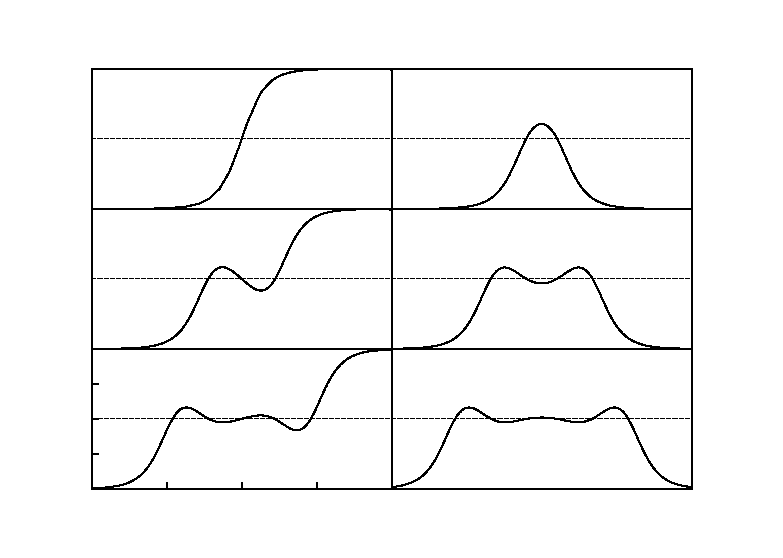
\includegraphics{graphics/Harmonic_static_to_multiplot}}%
    \gplfronttext
  \end{picture}%
\endgroup

  \caption{The first six non-trivial harmonic maps between spheres
    (solutions to \eqref{eq:f_psi_EL}). $\ln(\tan(\psi/2))$ scale of
    the abscissa is due to the fact that each $f_n$ is steeper near
    the boundaries.}
  \label{fig:Harmonic_maps}
\end{figure}

In \cite{Corlette2001} the authors proved that $f_n$ has index $n$
(there are $n$ negative eigenvalues of the Hessian of the
energy). From the last statement it follows that there are no local
minima of $E(f)$ apart from $f_0$. As we will need the following
property later on we introduce it in a form of the theorem.
\begin{theorem}[Wald, Corlette\cite{Corlette2001}]
  \label{thm:harmonic-map-index}
  There are no local minima of $E(f)$ apart from $f=n\pi$.
\end{theorem}
\begin{proof}
  This can also be proved by showing that for each $n>0$, $f_n$ there
  is at least one direction $v$ for which the Hessian is negative
  \begin{align}\label{eq:30}
    \begin{split}
      \delta^2E(f_n)(v,v) &=\int_0^{\pi} \left(
        v'^2+(k-1)\frac{\cos2f_n}{\sin^2\psi}v^2 \right)\sin^{k-1}\psi
      d\psi\\
      &=(v,\mathcal{L}_n v),
    \end{split}\\
    \mathcal{L}_nv&=-\frac{1}{\sin^{k-1}\psi}\left(\sin^{k-1}\psi
      v'\right)'+(k-1)\frac{\cos2f_n}{\sin^2\psi}v.
  \end{align}
  It turns out that the conformal Killing on $S^k$
  field
  \begin{align}
    \label{eq:31}
    K=\sin\psi\frac{\partial}{\partial\psi}
  \end{align}
  related to \eqref{eq:13} generates such $v$, namely for $v=\sin\psi
  f_n'(\psi)$ by \eqref{eq:strange_variation} we have
  \begin{align}
    \label{eq:32}
    \mathcal{L}_n v&=(2-k)v\\
    \delta^2 E(f_n)(v,v)&=(v,\mathcal{L}_n v)=(2-k)\lVert v\rVert^2<0.
  \end{align}
  This construction does not apply for $n=0$ in which case $v=0$.
\end{proof}

%%% Local Variables:
%%% mode: latex
%%% TeX-master: "master"
%%% End:


\section*{Stability of the equatorial map}

The stability of the equatorial map is governed by the eigenvalues of
\begin{align}
  \label{eq:4}
  -v''-(k-1)\cot\psi v'-\frac{k-1}{\sin^2\psi}v=\Lambda v.
\end{align}
According to our convention, $\Lambda<0$ corresponds to unstable
direction. The above equation can be considered as an eigenproblem of
the operator $L$ such that
\begin{align}
  \label{eq:5}
  Lv=-v''-(k-1)\cot\psi v'-\frac{k-1}{\sin^2\psi}v.\\
  \D{L}=\{C^\infty_0(0,\pi)\}
\end{align}
(TODO:explain $L$ symmetric) where $C^\infty_0(0,\pi)$ is the set of
infinitely differentiable functions with support away from $0$ and
$\pi$. The Hilbert space in this case is
$L^2([0,\pi],\sin^{k-1}\psi)$. We can utilize the unitary map
$U:L^2([0,\pi],\sin^{k-1}\psi)\ra L^2([0,\pi])$ such that
$U:f(\psi)\ra f(\psi)\sin^{(k-1)/2}\psi$. $U$ maps $C_0^\infty(0,\pi)$
onto itself and transforms the middle term in \eqref{eq:5} into the
potential term
\begin{align}
  \label{eq:7}
  ULU^{-1}=\left(
    -\frac{d^2}{d\psi^2}+V(\psi)-\frac{3}{2}(k-1)\right)\\
  V(\psi)=\frac{1}{4}(k-7)(k-1)\cot^2\psi.
\end{align}
(Unitary maps leave the eigenvalues $\Lambda$ untouched.) We will get
rid of the constant potential term by defining
\begin{align}
  \label{eq:8}
  \lambda=\Lambda+\frac{3}{2}(k-1).
\end{align}
The eigenproblem changed its form to
\begin{align}
  \label{eq:9}
  Kf=\lambda f
\end{align}
or
\begin{align}
  \label{eq:15}
  -f''+V(\psi)f=\lambda f.
\end{align}
Now as the proper dynamics may be generated only by the self-adjoint
operators we will have to verify weather $K$ (and thus $L$) is a
self-adjoint operator.
\begin{theorem}
  $K$ is essentially self-adjoint iff $4-2\sqrt{3}\ge
  k\ge4+2\sqrt{3}$.
\end{theorem}
\begin{proof}
  We will use the Weyl's limit-point/limit-circle criterion to
  determine the deficiency indices of $K$ (see [Simon,Reed,theorem
  X.7]). To do that, we have to investigate the number of solutions to
  the equations
  \begin{align}
    \label{eq:12}
    -f''+Vf=if\\
    -f''+Vf=-if
  \end{align}
  As $K$ commutes with complex conjugation, by the von Newmann's
  theorem, it has equal deficiency indices and it is enough to
  consider solutions to
  \begin{align}
    \label{eq:14}
    -f''+Vf=if
  \end{align}
  with $f\in\LSq$. As $V$ is infinitely differentiable at every point
  $\psi$ from $(0,\pi)$, it is enough to check the number of
  admittable solutions at $\psi=0$ and at $\psi=\pi$. But the
  potential $V$ is symmetric under the reflection $\psi\ra\pi-\psi$
  and thus so is $K$, therefore the exponents at $\psi=0$ and at
  $\psi=\pi$ are the same. At $\psi=0$ the possible solutions to
  \eqref{eq:14} behave as $\psi^{\gamma_+}$ and $\psi^{\gamma_-}$ with
  \begin{align}
    \label{eq:10}
    \gamma_\pm=\frac{1}{2}\left(1\pm\sqrt{k^2-8k+8}\right).
  \end{align}
  For $\psi^{\gamma_-}$ not to be in $\LSq$ we need $4-2\sqrt{3}\ge
  k\ge4+2\sqrt{3}$, so for such $k$ there would be only one solution
  to \eqref{eq:14} at each boundary. By the Weyl's limit-point,
  limit-circle criterion we obtain the claimed theorem.
\end{proof}
As the byproduct of this proof we get the following corollary
\begin{corollary}
  The deficiency indices of $K$ are $<2,2>$ for
  $k\in(4-2\sqrt{3},4+2\sqrt{3})$.
\end{corollary}
The exponents of the solutions to \eqref{eq:15} at $\psi=0$ can be
written in the more compact form by defining
\begin{align}
  \label{eq:18}
  \alpha=\frac{1}{2}\sqrt{k^2-8k+8},\\
  \gamma_\pm=\frac{1}{2}\pm\alpha.
\end{align}
As $\alpha$ can be either real or purely imaginary depending on $k$ we
shall further split our problem into three possible sets of $k$
\begin{align}
  \label{eq:20}
  \Gamma_1&=(-\infty,4-2\sqrt{3}]\cup[4+2\sqrt{3},\infty),\\
  \Gamma_2&=(4-2\sqrt{3},4-2\sqrt{2}]\cup[4+2\sqrt{2},4+2\sqrt{3}),\\
  \Gamma_3&=(4-2\sqrt{2},4+\sqrt{2}).
\end{align}
For $\Gamma_1$ $K$ is essentially self-adjoint, and thus admits the
dense set of eigenvectors. For $k\in\Gamma_2$ the exponents are real,
and for $k\in\Gamma_3$ the exponents have imaginary parts which
generate oscillations around the origins.\\

As $\Gamma_i$ for different $i$ need different treatment we continue
the stability analysis for each of them in three separate sections.

%%% Local Variables:
%%% mode: latex
%%% TeX-master: "master"
%%% End:


\subsection{The case $k\in\Gamma_1$}
\label{sec:case-kingamma_1}

As $K$ is already self-adjoint we shall proceed to solving the
eigenproblem
\begin{align}
  \label{eq:21}
  -f''(\psi)+\frac{1}{4}(k-7)(k-1)\cot^2\psi f(\psi)=\lambda f(\psi)
\end{align}
The general solutions to above ODE are the conical functions
\begin{align}
  \label{eq:1}
  f_\lambda&=\sqrt{\sin\psi}
  \left(AP_{\beta}^{\alpha}(\cos\psi)+BP_{\beta}^{-\alpha}(\cos\psi)\right)\\
  \alpha&=\frac{1}{2}\sqrt{k^2-8k+8}>0\\
  \beta&=\frac{1}{2}\left(-1+\sqrt{4\alpha^2-1+4\lambda}\right).
\end{align}
(TODO: $\Lambda_m>0$) As $\sqrt{\sin\psi}P_\beta^{\alpha}(\cos\psi)\sim\psi^{1/2-\alpha}$
grows too rapidly at $\psi=0$, we set $A=0$. We now analyse the
behaviour at $\psi=\pi$ by expanding $P_\beta^{-\alpha}$ around
$\cos\pi=-1$
\begin{align}
  \label{eq:2}
  &P_\beta^{-\alpha}(z)=\\
  &\frac{2^{\alpha/2}\Gamma(\alpha)}{\Gamma(\alpha-\beta)\Gamma(\beta+\alpha+1)}
  (z+1)^{-\alpha/2}(1+\mathcal{O}((z+1)))\\
  &-\frac{1}{\pi}2^{-\alpha/2}\sin(\pi\beta)\Gamma(-\alpha)
  (1+z)^{\alpha/2}(1+\mathcal{O}((z+1)))
\end{align}
We obtain the quantization of $\lambda$ by setting the coefficient in
the first term to zero. This can be achieved only by setting $\beta$
so that one of the functions $1/\Gamma(z)$ will zero, which induces
$\beta\in\R$. But then $\beta+\alpha+1>0$ and the only possible zeroes
are for
\begin{align}
  \label{eq:3}
  \alpha-\beta=-m\\
  m\in\mathbb{N}_0
\end{align}
which gives rise to the following quantization of $\Lambda$
\begin{align}
  \label{eq:6}
  \Lambda_m&=m^2+m(1+2\alpha)+\alpha+2-\frac{3}{2}k\\
  &=(m+\frac{1}{2}(1+2\alpha))^2-\frac{1}{4}(k-1)^2\\
  &=(m+\alpha+1-\frac{k}{2})(m+\alpha+\frac{k}{2})\\
  &>0\quad\text{for } k\in\Gamma_1 (TODO, not true!!)
\end{align}
so, the equatorial map is stable for $k\in\Gamma_1$.  The general
solutions to \eqref{eq:21} form an orthogonal basis
\begin{align}
  \label{eq:11}
  f_m(\psi)=\sqrt{\sin\psi}P_{\alpha+m}^{-\alpha}(\cos\psi)
\end{align}
The sum of the coefficients $\alpha$ and $\alpha-m$ is an non-positive
integer $-m$ which means that $P_{\alpha+m}^{-\alpha}(z)$ and
$P_{\alpha+m}^{-\alpha}(-z)$ are linearly dependent, therefore
$f_m(\psi)$ is either, symmetric or antisymmetric
w.r.t. $\psi\ra\pi-\psi$.


%%% Local Variables:
%%% mode: latex
%%% TeX-master: "master"
%%% End:


\subsection{The case $k\in\Gamma_2$}
\label{sec:case-kingamma_2}

Under such condition for $k$, the domain of $K^*$ is the set of
functions from $\LSq$ and both solutions to \eqref{eq:14} are
valid. However, one of the solutions blows-up at $\psi=0$ as
$\psi^{1/2-\alpha}$ while the other one tends to zero as
$\psi^{1/2+\alpha}$, the same happens at $\psi=\pi$. It seems natural,
to select the self-adjoint extension which would allow only the
eigenvectors which fall off to zero at $\psi=0$ and $\psi=\pi$.
To achieve this we set the extended domain of $K$ to be
\begin{align}
  \label{eq:13}
  \D{K_2}=\{f\in C^\infty(0,\pi)|\quad f(0)=f(\pi)=0\}.
\end{align}
With respect to the above domain, the domain of the operator and its
adjoint have to be the same and thus $K_2=K_2^*$. It can be
seen by utilizing the fact, that for every vector $g\in\D(K_2^*)$
and $f\in\D(K_2^*)$ we shall have
\begin{align}
  \label{eq:17}
  0&=(g,K_2 f)-(K_2^*g,f)\\
  &=f'(\pi)g(\pi)-f(\pi)g'(\pi)+f'(0)g(0)-f(0)g'(0)\\
  &=f'(\pi)g(\pi)-f'(0)g(0).
\end{align}
This implies $g(0)=g(\pi)=0$. Thus $K_2$ is one of the possible
self-adjoint extensions of $K$. As $\alpha$ is real for $k\in\Gamma_2$
the same reasoning as in \ref{sec:case-kingamma_1} holds and we find
the eigenvectors of $K_2$ to be the same which is another argument
behind choosing such extension. Such selection of the domain however,
produces self-adjoint extension only for $\alpha>1/2$ for which one of
the solutions blows up at $0$ and for the special case $k=7$ and $k=1$
for which $\alpha=1/2$ and one of the solutions is constant near the
boundaries.

As a matter of fact if we had chosen the domain \eqref{eq:13} in the
beginning we would have not reached the necessity of extending $K$ for
$\Gamma_2$. However, we have seen that such choice of the extension is
not an unique one thus without continuity in eigenvalues w.r.t $k$ as
a motivation we would not have any justification in our choice of
$K_2$. Another motivation is that the presence of any admixture of the
modes with singular behaviour at the boundaries in the spectrum would
produce, during the dynamical evolution, the singular behaviour even
for initial data without a singularities at the boundaries.


% To
% achieve this we have to calculate more explicitly how the choice of
% the possible extension of $K$, lets say $T$,
% \begin{align}
%   \label{eq:4}
%   T=-\frac{d^2}{d\psi^2}+V(\psi)
% \end{align}
% influences the domain of its adjoint. We have introduced the new
% letter $T$\\

% For vectors $f\in\D{T}$ and $g\in\D{T^*}$ we have
% \begin{align}
%   \label{eq:1}
%   (g,Tf)-(T^*g,f)=W(f,g)(\pi)-W(f,g)(0)=0.
% \end{align}
% Where $W(f,g)$ is the Wrońskian determinant for $f$ and $g$:
% \begin{align}
%   \label{eq:3}
%   W(f,g)(\psi)=f'(\psi)g(\psi)-f(\psi)g'(\psi)
% \end{align}
% We are considering the functions which possibly blow-up at $\psi=0$ or
% $\psi=\pi$ so we have to put limits into the formula
% \begin{align}
%   \label{eq:2}
%   (g,Tf)-(T^*g,f)=\lim_{\psi\ra\pi}W(f,g)(\psi)-\lim_{\psi\ra0}W(f,g)(\psi).
% \end{align}
% Assume, that $f\in\D{T}$ behaves as $\psi^{1/2+\delta_1}$ near
% $\psi=0$, and analogously $\D{T^*}\ni g\sim\psi^{1/2+\delta_2}$ for some
% real $\delta_1$ and $\delta_2$. Then
% \begin{align}
%   \label{eq:6}
%   W(f,g)(\psi)\sim(\delta_1-\delta_2)\psi^{\delta_1+\delta_2}.
% \end{align}
% The requirement for the Wrońskian to vanish in the limit $\psi\ra0$ is
% \begin{align}
%   \label{eq:7}
%   \delta_1+\delta_2>0\quad\text{or}\quad\delta_1=\delta_2.
% \end{align}
% We are interested in the case, where the singular eigenfunctions are
% not allowed to show up in the domain of $T$, so we set
% $\delta_1=\alpha>0$ and the second condition in \eqref{eq:7} is
% included in the first one. Thus the domain of

% The similar formula can be derived for


% This can be done, by expanding the
% domain of $K$ to the set of functions which do not grow faster than
% $\psi^{1/2+\alpha}$ at $\psi=0$ and $(\pi-\psi)^{1/2+\alpha}$ at
% $\psi=\pi$.
% \begin{align}
%   \label{eq:16}
%   D_1=\{f\in C^\infty(0,\pi)|\quad
%   \forall{\epsilon>0}\exists{M>0}:|f(\psi)|+|f(-\psi)|\}.TODO
% \end{align}
% With such domain, we expect

% The fact that both solutions belong to the $\LSq$

% In this case, the imposing self-adjoint extension
% is one for which we admit only solutions behaving nicely at $\psi=0$
% and at $\psi=\pi$, thus the set
% \begin{align}
%   \label{eq:16}
%   \{f\in C^\infty(0,\pi)|\quad f(0)=f(\pi)=0\}.
% \end{align}

% This choice of the domain guarantees that the solutions

% , as the deficiency indices pair is
% $<2,2>$, we end up with the possible self-adjoint extensions of $K$
% parametrized by $U(2)$.


% However, we can simplify the situation by admitting only
% symmetric or antisymemtric perturbations equivalent to considering the
% operators $L_+$ and $L_-$ for which respective domains are
% $\D(L_+)=\{f\in C^\infty(0,\pi)|\quad f(\psi)=f(-\psi)\}$ and
% $\D(L_-)=\{f\in C^\infty(0,\pi/2)|\quad f(\psi)=-f(-\psi)\}$. $L_+$ and
% $L_-$ when considered



% a bit we shall impose some arbitrary conditions on the
% domain of $K^*$, by restricting it to functions which are symmetric or
% antisymmetric. Such restricition is motivated by the following
% chapters, where we focus on symmetric or antisymmetric solutions to
% \eqref{eq:en_flow}. Let us introduce $K_+$ and $K_-$ each acting on
% either symmetric or antisymmetric subspaces of $C_0^\infty(0,\pi)$.

% By the similar reasoning as in (Thm1) we conclude, that each, $K_1$
% and $a$

%%% Local Variables:
%%% mode: latex
%%% TeX-master: "master"
%%% End:


\subsection{Case $k\in\Gamma_3$}
\label{sec:case-kingamma_3}

TODO:whole section\\

When the domain \eqref{eq:13} from section \ref{sec:case-kingamma_2}
no longer produces the self-adjoint extension we shall use other means
to present a suitable self-adjoint extension. As mentioned in the
previous section, the natural choice of the domain led us to the
continuity of the eigenvectors and eigenvalues with varying $k$ for
$\Gamma_1\cup\Gamma_2$. We shall now choose one of the self-adjoint
extension by expanding the continuity condition to $\Gamma_3$. We want
the set
\begin{align}
  \label{eq:22}
  f_m(\psi)=\sqrt{\sin\psi}P_{\alpha+m}^{-\alpha}(\cos\psi)
\end{align}
to span the domain of the possibly self-adjoint operator $K_3$. The
choice \eqref{eq:13} is not the right one, because its adjoint allows
both solutions as both of them fall off to zero at the edges.

%%% Local Variables:
%%% mode: latex
%%% TeX-master: "master"
%%% End:


\subsection{Case $k\in\Gamma_4$}
\label{sec:case-kingamma_4}

TODO: whole section\\

\begin{itemize}
\item $K$ is unbounded
\item self-adjoin extensions do exist
\item $K$ has deficiency indices $<2,2>$
\item There is no obvious way to obtain the eigenvalues from the given
  extension (complicated implicit relation)
\end{itemize}

%%% Local Variables:
%%% mode: latex
%%% TeX-master: "master"
%%% End:


% \section*{Stability of equatorial map}

% For $f$ to extremalize the energy it is required that
% \begin{gather}\label{eq:el}
%   \frac{1}{\sin^{k-1}\psi}\big(\sin^{k-1}\psi
%   f'\big)'-\frac{k-1}{2}\frac{\sin 2 f}{\sin^2\psi}=0.
% \end{gather}

% TEST:
% By applying the standard linearization procedure around $f_e=\pi/2$
% we obtain the eigenproblem
% \begin{align}
%   \label{eq:problem}
%   (L-\lambda)h=h''+(k-1)\cot(\psi)h'+\left(\frac{k-1}{\sin^2\psi}-\lambda\right)h=0.
% \end{align}
% The substitution $y=\sin^2\psi$, $g(y)=h(\arcsin(y^{1/2}))$ reveals
% the Fuchsian type equation with three regular singular points at $0$,
% $1$ and $\infty$:
% \begin{gather}
%   4y(y-1)g''+2(y+k(y-1))g'+(\lambda-\frac{k-1}{y})g=0.
% \end{gather}
% The general solution of the latter is of the form
% \begin{gather}
%   g=c_1\phi_1+c_2\phi_2\\
%   \phi_1(y)=y^{\frac{-4\alpha-k+2}{4}}{}_2F_1 \left(-\alpha-\beta+\frac{1}{4},-\alpha+\beta+\frac{1}{4};1-2\alpha;y\right)\\
%   \phi_2(y)=y^{\frac{+4\alpha-k+2}{4}}{}_2F_1 \left(\alpha-\beta+\frac{1}{4},\alpha+\beta+\frac{1}{4};1+2\alpha;y\right)\label{eq:sol}
% \end{gather}
% with
% \begin{gather}
%   \alpha=\frac{1}{4}\sqrt{k^2-8 k+8}\\
%   \beta=\beta(\lambda)=\frac{1}{4}\sqrt{(k-1)^2-4\lambda}.
% \end{gather}
% As we restrict ourselves to the real solutions we choose $c_1$ and
% $c_2$ in such a way that $g$ is real. Without further conditions,
% $\lambda$ can be any real number.


% The expansion of the solutions at $y=0$ yields
% \begin{gather}
%   \phi_1(y)=y^{\frac{-4\alpha-k+2}{4}}(1+O(y))\\
%   \phi_2(y)=y^{\frac{4\alpha-k+2}{4}}(1+O(y))
% \end{gather}


Stability of such mapping can be studied by investigating the energy
of linear perturbations of solutions of \eqref{eq:el}. The energy of
such perturbation is given by
\begin{gather}\label{eq:infE}
  \epsilon(h)=\delta^2E(f)(h,h)=\frac{1}{2}V(S^{k-1})\int_0^{\pi}\bigg(h'^2+(k-1)\frac{\cos
    2f}{\sin^2\psi }h^2\bigg)\sin^{k-1}\psi d\psi.
\end{gather}





The domain of $\epsilon$ is the set of functions for which
$\epsilon<\infty$, we will further denote such set
$\mathcal{D}(\epsilon)$ will further be denoted as $D_k$.


If we consider the lowest power of the Laurent series expansion of $h$
to be $\alpha$, the square integrability of its derivative requires
$\alpha>\alpha_{\text{crit}}$, where $\alpha_{\text{crit}}=1-k/2$. The
domain $D_k$ can be split into the symmetric and antisymmetric parts
without the loss of generality, such parts will be denoted as $D^+_k$
and $D^-_k$ respectively, which in turn lets us restrict the interval
$[0,\pi]$ to its half: $[0,\pi/2]$. Direct calculation gives us
\begin{gather}
  \epsilon(h)=-\frac{1}{2}(h,Lh)+\frac{1}{2}hh'\sin^{k-1}\psi\bigg|_0
\end{gather}
with
\begin{gather}
  (f,g)=\frac{1}{2}V(S^{k-1})\int_0^\pi f(\psi) g(\psi) \sin^{k-1}\psi d\psi,\\
  Lh=\frac{1}{\sin^{k-1}\psi}\big(h'\sin^{k-1}\psi\big)'-(k-1)\frac{\cos 2 f}{\sin^2\psi}h,\\
  (Lg,f)-(g,Lf)=gf\left(\log\frac{g}{f}\right)'\sin^{k-1}\psi\bigg|_0.
\end{gather}
We have left the boundary terms (with the value at $\pi/2$ equal to
$0$ for symmetric/antisymmetric subspaces) because they shall play an
important role in further discussion.

and the question of stability is brought to the eigenvalue problem for
symmetric operator $L$.\\

The mapping of our interest is $f(\psi)=\frac{\pi}{2}$, the eigenvalue
problem states that
\begin{gather}\label{eq:problem}
  (L-\lambda)h=h''+(k-1)\cot(\psi)h'+\left(\frac{k-1}{\sin^2\psi}-\lambda\right)h=0.
\end{gather}
The substitution $y=\sin^2\psi$, $g(y)=h(\arcsin(y^{1/2}))$ reveals
the Fuchsian type equation with three regular singular points at $0$,
$1$ and $\infty$:
\begin{gather}
  4y(y-1)g''+2(y+k(y-1))g'+(\lambda-\frac{k-1}{y})g=0.
\end{gather}
The general solution of the latter is of the form
\begin{gather}
  g=c_1\phi_1+c_2\phi_2\\
  \phi_1(y)=y^{\frac{-4\alpha-k+2}{4}}{}_2F_1 \left(-\alpha-\beta+\frac{1}{4},-\alpha+\beta+\frac{1}{4};1-2\alpha;y\right)\\
  \phi_2(y)=y^{\frac{+4\alpha-k+2}{4}}{}_2F_1 \left(\alpha-\beta+\frac{1}{4},\alpha+\beta+\frac{1}{4};1+2\alpha;y\right)\label{eq:sol}
\end{gather}
with
\begin{gather}
  \alpha=\frac{1}{4}\sqrt{k^2-8 k+8}\\
  \beta=\beta(\lambda)=\frac{1}{4}\sqrt{(k-1)^2-4\lambda}.
\end{gather}
First and foremost we are interested in the behavior at
$\psi\rightarrow0$. The series expansion reveals that
\begin{gather}
  \phi_1(y)=y^{\frac{-4\alpha-k+2}{4}}(1+O(y))\\
  \phi_2(y)=y^{\frac{4\alpha-k+2}{4}}(1+O(y))
\end{gather}
% First, one should notice that, for $\Im(\alpha)\ne0$, $y^\alpha$ is
% not integrable on $[0,1]$. This introduces the condition
% $k>2(2+\sqrt{2})$ or $k<2(2-\sqrt{2})$. The latter case shall not be
% considered as we assume $k\ge3$.
For $k>2(2+\sqrt{2})=k_{\text{crit}}\approx6.8284$ we have
$\frac{-4\alpha-k+2}{4}<\frac{\alpha_{\text{crit}}}{2}$, so for
$k>k_{\text{crit}}$ the first solution has to be discarded, also for
such $k$, we have $\Im{\alpha}=0$, thus there are no oscillations
around $y=0$. This makes the case $k>k_{\text{crit}}$ much easier to
solve and we shall take care of it in the following section.

\section*{Stability for $k>k_{\text{crit}}$}

At $y\rightarrow1$ the values of $h$ and
$h'$ are
\begin{align}
  h=g&
  \sim\frac{\Gamma(1+2\alpha)}{\Gamma\left(\frac{3}{4}+\alpha-\beta\right)\Gamma\left(\frac{3}{4}+\alpha+\beta\right)}+O(1-y),\\
  h'=2y^{1/2}(1-y)^{1/2}g'&
  \sim\frac{\left(\left(\frac{1}{4}+\alpha\right)^2-\beta^2\right)\Gamma(2+2\alpha)}{\Gamma\left(\frac{5}{4}+\alpha-\beta\right)\Gamma\left(\frac{5}{4}+\alpha+\beta\right)}+O(1-y)
\end{align}
The antisymmetry of $h$, requires that $h(\pi/2)=g(1)=0$, and this is
true iff $\beta^2=(m_1+3/4+\alpha)^2$ for
$m_1\in\mathbb{N}_0$. Similarly if $h'(\pi/2)$ vanishes then
necessarily $\beta^2=(m_2+5/4+\alpha)^2$ for $m_2\in\mathbb{N}_0$ (the
special case when numerator is zero is covered by the $m_2=1$). Both
formulas can be combined into $\beta^2=(\alpha+(3+2n)/4)^2$ for
$n\in\mathbb{N}_0$ with $n$ even for symmetric modes and odd for
antisymmetric ones. We can calculate $\lambda_n$ as
\begin{align}
  \lambda_n&=\frac{1}{2}(-\alpha(8n+12)+(3k-2n^2-6n-8))\\
  &=\frac{1}{4}(2n+4-k+\alpha)(2n+2+k+\alpha)
\end{align}

The noticeable fact is, that the only eigenvalues grater than zero are
for $n=0$ (antisymmetric solution), and as $k\rightarrow\infty$ one
has $\lambda_0= 2 + O(1/k)$ and $\lambda_1=-k+O(1)$. More generally,
the asymptotic of $\lambda$ w.r.t. $k$ is as follows
\begin{gather}
  \lambda_n=-nk+(n+1)(2-n)+O(1/k).
\end{gather}
(TODO: mention the special dimension $k=7$ where $\lambda_1=0$.)
Substituting eigenvalues to \eqref{eq:sol} and using the value of
\begin{gather}
%   \beta^-_m=3/4+m+\alpha\\
%   \beta^+_m=1/4+m+\alpha\\
  \beta_n=\beta(\lambda_n)=\frac{1}{4}(3+2n+4\alpha)
\end{gather}
we end up with the complete solution to \eqref{eq:problem}
\begin{gather}
%   h^-_m(\psi)=A\sin^{2\alpha+\frac{-k+2}{2}}\psi\sideset{_2^{}}{_1^{}}F(-\frac{1}{2}-m,1+m+2\alpha;1+2\alpha;\sin^2\psi),\\
%   h^+_m(\psi)=B\sin^{2\alpha+\frac{-k+2}{2}}\psi\sideset{_2^{}}{_1^{}}F(-m,\frac{1}{2}+m+2\alpha;1+2\alpha;\sin^2\psi),\\
  h_n(\psi)=C_n\sin^{\frac{4\alpha-k+2}{2}}\psi {}_2 F_1
  \left(-\frac{n+1}{2},\frac{n+1}{2}+\frac{1+4\alpha}{2};1+2\alpha;\sin^2\psi\right).
\end{gather}


For $k=7$ the solution turns out to be particularly simple, because the
factor $(1+4\alpha)/2=1$, and we can use the compactified form of
hypergeometric function
\begin{gather}
%   h^-_m(\psi)=A_m\sin^{-2}\psi \sideset{_2^{}}{_1^{}}F(-\frac{1}{2}-m,\frac{3}{2}+m;\frac{3}{2};\sin^2\psi)
%   =\frac{\sin((2+2m)\psi)}{(2+2m)\sin^3\psi},\\
%   h^+_m(\psi)=B_m\sin^{-2}\psi \sideset{_2^{}}{_1^{}}F(-m,1+m;\frac{3}{2};\sin^2\psi)
%   =\frac{\sin((1+2m)\psi)}{(1+2m)\sin^3\psi}.
  h_n(\psi)=C_n\sin^{-2}\psi
  {}_2F_1\left(-\frac{n+1}{2},\frac{n+1}{2}+1;\frac{3}{2};\sin^2\psi\right)
  =\frac{C_n}{n+2}\frac{\sin((n+2)\psi)}{\sin^3\psi},\\
  \lambda_n=(5+n)(1-n).
\end{gather}

% which can be compactified to

% \begin{gather}
%   h_k(\psi)=C_k\frac{\sin(k\psi)}{k\sin^3\psi}
% \end{gather}


\section*{Stability for $k<k_{\text{crit}}$}

$\phi_1=\bar{\phi_2}$ for $k<k_\text{crit}$ and $\lambda\in R$ (from
$\overline{F(a,b;c;y)}=F(\bar{a},\bar{b};\bar{c};\bar{y})$, and the
symmetry in $a$ and $b$, using the fact, that $\beta$ is purely real
or purely imaginary), with both, $\phi_1$ and $\phi_2$ integrable. For
$k>k_\text{crit}$ $\phi_2=\bar{\phi_2}$, and $\phi_1$ is not
integrable, the most general form of the real solution when
$k<k_\text{crit}$ is (with $\phi:=\phi_1$, and $a_1$, $a_2$ - real
parameters)
\begin{gather}
  g=a_1(\phi+\bar\phi)+i a_2(\phi-\bar\phi)
\end{gather}
For $L$ to be self-adjoint the boundary terms are of the form
(in $f$,$g$ - functions of $\psi$)
\begin{gather}
  (f'g-fg')\sin^{k-1}\psi\big|^\pi_0\sim \bigg(\ln \frac{f}{g}\bigg)'fg\sin^{k-1}\psi\big|_0^\pi
\end{gather}
and have to vanish, which in the case of $k<k_\text{crit}$ reduces to
the requirement, that all eigenfunctions have linearly-dependent
asymptotics at $0+$ (this can be achieved, because the leading
asymptotics at $0+$ does not depend on $\lambda$) and, as $a1$ and
$a2$ are chosen globally, for the whole domain of $g$, the domain of
self-adjoint operator $L$ is therefore parametrized by the ``phase''
parameter $\theta\in[0,\pi]$ of $(a_1,a_2)$, which is an element of
$RP^1\sim^?U(1)$ (which agrees with the von Neuman theorem for
non-unique self-adjoint extensions), and the behaviour of the solutions
for fixed $\theta$ are dependent of $\lambda$ only. This means that
for given $\theta$ we can quantize $\lambda$ using boundary conditions
as for $k>k_\text{crit}$ (symmetricity/antisymmetricity). This leaves
us with the family of sets of eigenvalues $\{\lambda_m\}$ parametrized
by the $\theta$. Conversely, for arbitrary large $\lambda$, there
exists $\theta$ for which the boundary values are fulfilled (unless,
$\phi(1)\ne0$). This becomes obvious if one uses the relation for
$g_\lambda(1)$ and $\theta$:
\begin{gather}
  g_\lambda(1)=a_0(\phi_\lambda(1)
  e^{i\theta}+\overline{\phi_\lambda(1)} e^{-i\theta})=2a_0\Re
  (\phi_\lambda(1) e^{i\theta})=0
\end{gather}
and from continuity of $\phi_\lambda(1)$ in $\lambda$ two situations
may occur in the limit of $\lambda\rightarrow\infty$. Either, there is
a limiting value of $\theta_0$ (from which it results in self-adjoint
bounded from above extensions ), or there is no limiting value of
$\theta$ in which case $\theta$ is expected to go round the $[0,\pi]$
interval infinitely many times in which case arbitrary $\theta$ is
``crossed'' infinitely many times with the value of $\lambda$
increasing at each round, and we and up with extension unbound from
top for any $\theta$. The unboundness from below can be shown in the
same way of reasoning, or using the Sturm-Liouville theorem, but is of
no particular use.

%%% Local Variables:
%%% mode: latex
%%% TeX-master: "master"
%%% End:


\section*{Stability of the ground states}

Given the solution $f_0=0$ we consider the small perturbation of the
form $f=f_0+e^{\lambda t} v$ with $v<<1$. The equation for $v$ is thus
of the form
\begin{align}\label{eq:f0_L}
  v''+(k-1)\cot\psi v'-(k-1)\frac{v}{\sin^2\psi}=\lambda v.
\end{align}
The critical exponents at $\psi=0$ are $1$ and $1-k$. The latter will
be rejected because the finitness of the energy condition yields that
the exponent $\alpha$ at $\psi=0$ has to fulfill
$\alpha>1-\frac{k}{2}$. Now when we know that $v$ and $v'$ are square
integrable we can multiply \eqref{eq:f0_L} by $\sin^{k-1}\psi v$ and
integrate on the interval $[0,\pi]$ to get
\begin{align}
  \lambda\int_0^\pi v^2w d\psi=-\int_0^\pi\left(v'^2+\frac{k-1}{\sin^2\psi}v^2\right)\sin^{k-1}d\psi.
\end{align}
All the terms under the integrals are positive for $v\ne0$ so
$\lambda<0$ and $f_0$ is linearly stable.\\

We use the similar reasoning for $f_1=\psi$ to get same critical
exponents and
\begin{align}
  \label{eq:f1_lambda}
  \lambda\int_0^\pi v^2w d\psi=-\int_0^\pi\left(v'^2+(k-1)\frac{\cos2\psi}{\sin^2\psi}v^2\right)\sin^{k-1}d\psi.
\end{align}
This time the term $\cos2\psi$ can change its sign, but if we restrict
to perturbations that are antisymmetric around the point $\pi/2$ the

%%% Local Variables:
%%% mode: latex
%%% TeX-master: "master"
%%% End:


\section*{Blow-up}

As we mentioned, apart from the first global attractor $f_0$ there
exists its image by the reflection symmetry $\bar{f}_0=\pi$ which is
also a global minimum of the energy. It turns out that before reaching
the second attractor the spatial derivative of the solution blows up
at the edges of the interval $[0,\pi]$. As the blow up is localized,
let's say at $\psi=0$, we can rewrite \eqref{eq:en_flow} up to first
corrections in $\psi$
\begin{align}
  \label{eq:2}
  \partial_t h=f''+\frac{(k-1)}{\psi}f'-\frac{k-1}{2}\frac{\sin2h}{\psi^2}.
\end{align}
This equation has the scaling symmetry of the form
$\psi\ra\lambda\psi$ and $t\ra\lambda^2t$ therefore we use the
self-similar ansatz of the form


% We shall now answer the question
% of how the convergence to this attractor is realized for initial data
% $g$ consistent with \eqref{eq:en_flow} for $\delta=0$
% \begin{align}
%   \label{eq:2}
%   f(\psi,0)=g(\psi)\\
%   g(0)=g(\pi)=0.
% \end{align}
% It is clear, that for $g$ close enough to $\pi$ in $L^2([0,\pi])$ the
% solution can have arbitrary small energy and thus should converge to
% $\pi$. However, the boundary conditions prevent the solution from
% converging to $\bar{f}_0$ uniformly,

% First of all, we notice that there exist continous functions $g$ of
% arbitrary small energy, yet close to $\pi$. Such functions are
% obtained by




%%% Local Variables:
%%% mode: latex
%%% TeX-master: "master"
%%% End:


\section{Bisection}
\label{sec:bisection}

% We will now use the heat flow \eqref{eq:en_flow} to implement the
% dynamical version of simple yet powerful technique called the mountain
% pass, which allows to prove the existence of the saddle point of the
% given functional. The intuition behind this technique is that given
% the path connecting two valleys which are separated by mountains,
% there has to be a point along that path from which if we have dropped
% a ball it won't fall into neither of the valleys, and thus it will has
% to roll down to some saddle point.\\

Although we already know that $f_2$ and $f_3$ are saddle points of
$E(f)$ we shall demonstrate in this section how to obtain them using
only the heat flow \eqref{eq:en_flow}.\\

% The implementation of this procedure to $H_+$ will look as follows.
Let us formally denote the basins of attraction of $0$ and $\pi$ as
$\Gamma(0)$ and $\Gamma(\pi)$ respectively. We say formally, because
the solutions to \eqref{eq:en_flow} will blow up (e.g. by Theorem
\ref{thm:Struwe}) before asymptotically converging to either of the
ground states. We start by choosing $g_+\in\Gamma(\pi)\cap H_+$ and
$g_+(0)=g_+(\pi)=0$. We now form a path $g_A\in H_+$ such that
\begin{align}
  \label{eq:93}
  g_A=A\cdot g_+,\quad A\in[0,1].
\end{align}
Obviously for $0\le A\ll1$, $g_A\in \Gamma(0)$, so the curve
intersects both, $\Gamma(0)$ and $\Gamma(\pi)$. As $\Gamma(\pi)$ and
$\Gamma(0)$ are disjoint open sets, the curve leading from one of them
into another has to contain the closed set which does not belong to
either of the open sets. By definition, initial data from this set
cannot fall into any of those attractors. This means that there is at
least one $A^*$ such that the flow starting from $g_{A^*}$ is not
going to converge to the global energy minimum. Still, for any initial
data the energy has to decrease along the flow and for $A=A^*$ it
cannot asymptotically decrease to $0$, so its infimum $E^*$ obeys
\begin{align}\label{eq:94}
  E^*=\inf_{t\ge0} E(t)>0
\end{align}
and hence, if $g_{A^*}$ does not blow up, the limiting values are
\begin{align}\label{eq:95}
  \lim_{t\ra\infty}E(t)=E^*>0,\quad \lim_{t\ra\infty}\frac{dE}{dt}(t)=0.
\end{align}
But, $dE/dt\ra0$ can happen only if $\partial_t f\ra0$ so
\begin{align}\label{eq:96}
  \lim_{t\ra\infty}f(t,\psi)=f^*(\psi)
\end{align}
which means, that $f^*$ is a symmetric solution to
\eqref{eq:f_psi_EL} with $E(f^*)=E^*$, different from the ground
states and, by construction, it is a saddle point in $H_+$. As $g_+$
was chosen to be generic, by such procedure we will obtain the saddle
point of the lowest index, namely $f^*=f_2$.\\

Analogous procedure can be applied to $H_-$ with $(\psi+g_-)\in
H_-\cap\Gamma(\pi-\psi)$, $g_-(0)=g_-(\pi)=0$ and
\begin{align}
  \label{eq:97}
  g_B=\psi+B\cdot g_-,\quad B\in[0,1]
\end{align}
to obtain $f_3$.\\



%%% Local Variables:
%%% mode: latex
%%% TeX-master: "master"
%%% End:


\section{Static solutions}
\label{sec:static-solutions}

\begin{align}
  \label{eq:19}
  f(t,\psi)=f_2(\psi)+C_1 e^{-\lambda_1 t}u_1(\psi)+C_2e^{-\lambda_2
    t}u_2(\psi)+\cdots\\
  f(t,\psi)=f_3(\psi)+D_1e^{-\kappa_1 t}v_1(\psi)+D_2e^{-\kappa_2 t}v_2(\psi)+\cdots
\end{align}


%%% Local Variables:
%%% mode: latex
%%% TeX-master: "master"
%%% End:


% \section*{Dimension $3\le k\le6$}

Equatorial map does not interfere with the global dynamics of the
system Apart from being linearly stable, $f_0$ and $\bar{f}_0$ are
separated (TODO: in what sense?) global minimas of energy functional
($E(f_0)=E(\bar{f}_0)=0$), so from the monotonicity of the energy we
would expect that for generic initial data the solution should fall
into one of such attractors. However, we shall see that in the phase
space there exists the set of solutions that fall to neither of the
attractors and thus imply the existence of nontrivial solution to
\eqref{eq:f_psi_EL}.


%%% Local Variables:
%%% mode: latex
%%% TeX-master: "master"
%%% End:


\clearpage
\chapter{Useful identity}
\label{cha:Identity}

Given the E-L equations
\begin{align}
  \frac{1}{w}\left(wf'\right)'+V(f,x)=0
\end{align}
the second variation in the direction $v=gf'$, for $g$ arbitrary, can
be written as
\begin{align}\label{eq:strange_variation}
  \frac{1}{w}\left(wv'\right)+\frac{\partial V}{\partial
    f}v=\frac{1}{g}\left[\left(\left(\frac{g}{w}\right)'w
  \right)'v-\frac{\partial}{\partial x}\left(g^2 V(f,x)\right)\right]=A(x)v+B(f,x).
\end{align}
Where we have differentiated the E-L equation, multiplied it by $g$
and used the fact that
\begin{align}
  \frac{1}{w}\left(w(gf')'\right)'-g\left(\frac{1}{w}(gf')'\right)'
  =\left(\left(\frac{g}{w}\right)'w \right)'f'-2g'V(f,x).
\end{align}
% In all cases considered in this thesis we have $A(x)=const$ and
% $B(f,x)=0$.
% This cannot be a coincidence and such situation has to
% reflect some particular symmetry of the E-L equation. Worth noticing
% is the fact that in all cases $wg$ is eigenfunction of the laplacian

% \begin{align}
%   \frac{1}{w}\left(w(wg)'\right)'=\lambda wg
% \end{align}

% to some particular $\lambda$ which is also the eigenvalue of the first
% perturbation operator. Moreover $B=0$ implies that
% $V(f,x)=U(f)/g^2(x)$.

\chapter{Numerical methods}
\label{cha:numerical-methods}

\section{Method of lines}
\label{sec:method-lines}

In order to solve the Cauchy problem
\begin{align}
  \label{eq:118}
  \partial_t f=\tau(f),\quad f(0,\psi)=g(\psi)
\end{align}
we discretize the spatial domain in a uniform way to create the grid
of $N$ points
\begin{align}
  \label{eq:107}
  \psi_i=\frac{i-1}{N-1}\pi\in[0,\pi],\quad i\in{1,\dots,N}.
\end{align}
To each point we assign a function of time $f_i(t)$, and we denote the
set of $f_i$ as a vector $\vec{f}\in\mathbb{R}^N$. Then, the solution
to \eqref{eq:118} at points $\psi_i$ can be approximated by $f_i(t)$
if $\vec{f}$ is a solution to the following ordinary differential
equation
\begin{align}
  \label{eq:121}
  \frac{d \vec{f}}{dt}=\hat{\tau}(\vec{f}),\quad f_i(0)=g(\psi_i).
\end{align}
The map $\vec{\tau}:\mathbb{R}^N\ra \mathbb{R}^N$ is a discretized
approximation of $\tau$. As $\tau=\tau(f,\partial_\psi
f,\partial_{\psi\psi} f)$ it is sufficient to choose the
differentiation schemes approximating the first and second
derivatives. We choose the following discretizations of derivatives
called the three point stencil
\begin{align}
  \label{eq:123}
  \partial_\psi f\big|_{\psi_i}\approx D_i\vec{f}=\frac{1}{2h}(f_{i+1}-f_{i-1}),\\
  \partial_{\psi\psi} f\big|_{\psi_i}\approx D_i^2\vec{f}=\frac{1}{h^2}(f_{i+1}-2f_i+f_{i-1}),
\end{align}
where $1\ge i\ge N-1$. We do not define the $D_0$, $D_N$ etc. because
the boundary values imply $df_0/dt=0$ and $df_N/dt=0$ so we don't need
the approximations of $\tau(f)$ at points $\psi_0$ and $\psi_N$. The
above schemes are of order $2$ and $1$ respectively, which means that
\begin{align}
  \label{eq:124}
  \partial_\psi f\big|_{\psi_i}= D_i\vec{f}+\mathcal{O}(h^2),\\
  \partial_{\psi\psi} f\big|_{\psi_i}= D_i^2\vec{f}+\mathcal{O}(h).
\end{align}
With such choice of differentiation schemes we end up with a following
form of \eqref{eq:121}
\begin{align}
  \label{eq:125}
  \frac{d f_i}{dt}=\tau(f_i,D_i\vec{f},D_i^2\vec{f}),\quad f_i(0)=g(\psi_i).
\end{align}
We solve the above equation using a Runge-Kutta method with adaptive
step size described in the next section.

\section{Time marching method}
\label{sec:time-marching-method}

To approximate the solution to the initial value problem for ordinary
differential equation
\begin{align}
  \label{eq:114}
  y'(t)=f(t,y(t)),\quad y(0)=y_0
\end{align}
where $y\in \mathbb{R}^N$ and
$f:\mathbb{R}\times\mathbb{R}^N\ra\mathbb{R}^N$ we use the explicit
Runge-Kutta method with $s$ intermediate steps which approximates
$y_{n+1}=y(t_{n+1})$ by
\begin{align}
  \label{eq:115}
  y_{n+1}=y_n+h\sum_{i=1}^s b_i k_i,
\end{align}
where $k_i$ are the values of the intermediate steps given by
\begin{align}
  \label{eq:117}
  \begin{split}
    k_1 &= f(t_n,y_n), \\
    k_2 &= f(t_n+c_2 h, y_n+a_{21}k_1), \\
    & \ \ \vdots \\
    k_s &= f(t_n+c_s h, y_n + \sum_{j=1}^{s-1} a_{sj}k_j).
  \end{split}
\end{align}
The choice of the constants $c_i$, $a_{ij}$ and $b_i$ uniquely
determines a specific Runge-Kutta (RK) method, there is also a
systematical way of presenting those coefficient called the Butcher's
tableau (table \ref{tab:RKexplicit}).

\begin{table}[h]
  \begin{equation*}
    % \label{eq:19}
    \begin{array}{l | c c c c c}
      \rule{0pt}{2,3ex} 0      \quad &             &               &              &         &   \\
      \rule{0pt}{2,3ex} c_2    \quad & \quad a_{21}  &              &              &         &   \\
      \rule{0pt}{2,3ex} c_3    \quad & \quad a_{31}  & \quad a_{32}  &              &         &   \\
      \rule{0pt}{2,3ex} \vdots \quad & \quad \vdots & \quad \vdots & \quad \ddots &         &   \\
      \rule{0pt}{2,3ex} c_s    \quad & \quad a_{s1}  & \quad a_{s2}  & \quad \cdots & \quad a_{s,s-1} & \\[2,0ex] \hline
      \rule{0pt}{3,3ex}              & \quad b_{1}  & \quad b_{2}    & \quad \cdots & \quad b_{s-1}  & \quad b_{s}
    \end{array}
  \end{equation*}
  \caption{The Butcher tableau for the explicit Runge–Kutta method.}
  \label{tab:RKexplicit}
\end{table}

To calculate the solution in an efficient way one can vary the time
step size $\Delta t_n=t_{n+1}-t_{n}$ to decrease the number of
calculations per a unit of time, keeping the relative error constant
per unit of time. This is realized by combining two $s$-stage RK
methods, one of order $p$ and the other of order $p+1$ which use the
same intermediate values $k_i$, so having the same parameters $c_i$
and $a_{ij}$ but different $b_i$. The solutions are then approximated
by
\begin{align}
  \label{eq:105}
  y_{n+1}=y_n+h\sum_{i=1}^s b_i k_i,\quad y_{n+1}^*=y_n+h\sum_{i=1}^s
  b^*_i k_i,
\end{align}
where stars have been used to denote the coefficients of the method of
order $p+1$. The difference between $y_{n+1}$ and $y_{n}$ gives the
error estimate
\begin{align}
  \label{eq:106}
  \epsilon_i=|(y_{n+1})_i-(y_{n+1}^*)_i|=h\left|\sum_{j=1}^s(b_j-b_j^*)(k_j)_i\right|,\quad
  i\in\{1,\dots,N\}.
\end{align}
If the calculated error or too small compared with the desired error
level the method changes step accordingly to the algorithm described
in \cite{Galassi}. The method of our choice was embedded
Runge–Kutta–Fehlberg (RKF45) of order $4/5$ with the Butcher tableau
presented in table \ref{tab:rkf45}.

\begin{table}[h]
  \centering
  \begin{tabular}{l|lllll}
    0      &           &            &             &           &        \\
    1/4    & 1/4       &            &             &           &        \\
    3/8    & 3/32      & 9/32       &             &           &        \\
    12/13  & 1932/2197 & -7200/2197 & 7296/2197   &           &        \\
    1      & 439/216   & -8         & 3680/513    & -845/4104 &        \\
    1/2    & -8/27     & 2          & -3544/2565  & 1859/4104 & -11/40 \\\hline
    25/216 & 0         & 1408/2565  & 2197/4104   & -1/5      & 0      \\
    16/135 & 0         & 6656/12825 & 28561/56430 & -9/50     & 2/55
  \end{tabular}
  \caption{Butcher tableau for embedded Runge-Kutta-Fahlberg
    method. The lowest row contains $b_i^*$.}
  \label{tab:rkf45}
\end{table}



%%% Local Variables:
%%% mode: latex
%%% TeX-master: "master"
%%% End:


\bibliography{/home/pawel/library.bib}{}
\bibliographystyle{plain}

%%% Local Variables:
%%% mode: latex
%%% TeX-master: "master"
%%% End:


\end{document}

%%% Local Variables:
%%% mode: latex
%%% TeX-master: t
%%% End:
